% This is part of Un soupçon de mathématique sans être agressif pour autant
% Copyright (c) 2012
%   Laurent Claessens
% See the file fdl-1.3.txt for copying conditions.

%+++++++++++++++++++++++++++++++++++++++++++++++++++++++++++++++++++++++++++++++++++++++++++++++++++++++++++++++++++++++++++
\section{Définitions}
%+++++++++++++++++++++++++++++++++++++++++++++++++++++++++++++++++++++++++++++++++++++++++++++++++++++++++++++++++++++++++++

\begin{definition}
    Une fonction \defe{polynôme de degré $2$}{polynôme (de degré $2$)} est une fonction s'exprimant sous la forme 
    \begin{equation}
    f(x)=ax^2+bx+c
    \end{equation}
    où \( a\), \( b\) et \( c\) sont des nombres réels avec \( a\neq 0\). 
    
    La courbe représentative d'un polynôme de degré deux dans un plan orthonormé est une \defe{parabole}{parabole}.
\end{definition}

%---------------------------------------------------------------------------------------------------------------------------
\subsection{Symétries, tableau de variations}
%---------------------------------------------------------------------------------------------------------------------------

La parabole de la fonction \( f(x)=ax^2+bx+c\) (\( a\neq 0\)) est symétrique par rapport à la droite d'équation \( x=-\frac{ b }{ 2a }\), c'est à dire par rapport à la droite verticale en \( x=-b/2a\). Le \defe{sommet}{sommet (d'une parabole)} est le point d'abscisse 
\begin{equation}
x=-b/2a
\end{equation}
situé sur la parabole.

Deux paraboles avec leurs axes de symétries sont dessinées à la figure \ref{LabelFigParaboles}.
\newcommand{\CaptionFigParaboles}{Deux paraboles}
\input{Fig_Paraboles.pstricks}

Comment savoir si les branches de la paraboles \( ax^2+bx+c\) sont orientées vers le haut ou vers le bas ? La règle est simple : 
\begin{enumerate}
    \item
        si \( a>0\), alors elles sont tournées vers le haut;
    \item
        si \( a<0\), alors elles sont tournées vers le bas.
\end{enumerate}
Cette règle est facile à retenir en pensant par exemple à la parabole \( x^2+bx+c\) où \( b\) et \( c\) sont raisonnables. Si nous prenons \( x=1000\), alors \( x^2\) vaut un million alors que les deux autres termes ne valent que de l'ordre du mille. Il est alors clair que la branche part vers l'infini.

\vbox{  % Le problème est que ceci apparaît proche du bord inférieur de la page, du coup il saut de colonne avant mon \columnbreak et l'effet est merdé.
\begin{multicols}{2}
    
    Le tableau de variations pour une parabole \( f(x)=ax^2+bx+c\) avec \( a>0\) se présente ainsi :
\begin{equation*}
\begin{array}[h]{|c||ccccc|}
    \hline
    x&-\infty&&x_0=-b/2a&&\infty\\
    \hline
    &\infty&&&&\infty\\
    f(x)&&\searrow&&\nearrow&\\
    &&&f(x_0)&&\\
    \hline
\end{array}
\end{equation*}

  \columnbreak

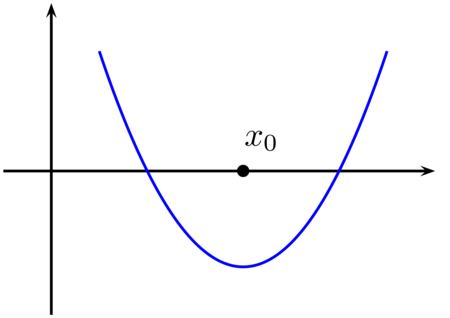
\includegraphics{Picture_FIGLabelFigParaboleHautMLbPQFPICTParaboleHautMLbPQF-for_eps.pdf}

\end{multicols}

}

\vbox{ 
\begin{multicols}{2}
    
    Le tableau de variations pour une parabole \( f(x)=ax^2+bx+c\) avec \( a<0\) se présente ainsi :
\begin{equation*}
\begin{array}[h]{|c||ccccc|}
    \hline
    x&-\infty&&x_0=-b/2a&&\infty\\
    \hline
    &&&f(x_0)&&\\
    f(x)&&\nearrow&&\searrow&\\
    &-\infty&&&&-\infty\\
    \hline
\end{array}
\end{equation*}


  \columnbreak

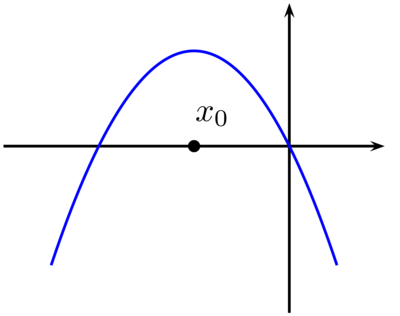
\includegraphics{Picture_FIGLabelFigParaboleBasfKtFCNPICTParaboleBasfKtFCN-for_eps.pdf}
\end{multicols}

}

%+++++++++++++++++++++++++++++++++++++++++++++++++++++++++++++++++++++++++++++++++++++++++++++++++++++++++++++++++++++++++++
\section{Tracer une parabole dont l'équation est connue}
%+++++++++++++++++++++++++++++++++++++++++++++++++++++++++++++++++++++++++++++++++++++++++++++++++++++++++++++++++++++++++++

Maintenant que les symétrie de la paraboles sont sont connues, il devient relativement facile d'en dessiner. Il est important d'être capable de tracer à main levée une courbe approximative passant par quelque points connus. SANS CALCULATRICE\footnote{Si vous me permettez une analogie, utiliser une calculatrice pour faire des études de fonctions, c'est comme utiliser un anti douleur pour améliorer ses performances sportives.}.

La méthode pour tracer la courbe représentative de \( f(x)=ax^2+bx+c\) se décompose en les pas suivants.
\begin{enumerate}
    \item
        D'abord il faut trouver le sommet de la parabole en utilisant la formule 
        \begin{equation}
            x_0=-\frac{ b }{ 2a }.
        \end{equation}
        Le somme est alors le point \( S=\big( x_0,f(x_0) \big)\).
    \item
        Tracer la droite verticale passant par le sommet; ce sera l'axe de symétrie.
    \item
        Dresser le tableau de variations de \( f\) en regardant le signe de \( a\). Si \( a\) est positif, le sommet sera le creux de la courbe; si \( a\) est négatif, alors le sommet sera un pic du graphique.
    \item
        Calculer quelque valeurs autour du sommet, par exemple \( x=0\), \( x=\pm1\).
    \item
        Tracer une belle courbe passant par les points calculés, ayant le bon axe de symétrie et le bon sommet.
\end{enumerate}

\begin{example}
    Traçons la courbe représentative de \( f(x)=x^2\). Ses paramètres sont \( a=1\), \( b=0\), \( c=0\); son axe de symétrie est donc \( x=0\), c'est à dire l'axe des ordonnées. Son sommet est le point \( S=(0,0)\) et le graphe passe par les points \( (-2,4)\), \( (-1,1)\), \( (0,0)\), \( (2,4)\). En repérant ces points sur la feuille, le tracé est aisé.

    Attention : c'est une courbe qui monte assez fort. Elle est tracée sur la figure \ref{LabelFigbDdpfh}.
\newcommand{\CaptionFigbDdpfh}{La courbe \( x\mapsto x^2\).}
\input{Fig_bDdpfh.pstricks}

\end{example}

\begin{example}
    Soit à tracer la courbe de \( f(x)=x^2-4x+3\).
    \begin{enumerate}
        \item
            Nous identifions \( a=1\), \( b=-4\), \( c=3\). 
        \item
            L'abscisse du sommet est \( x_0=-b/2a=\frac{ 4 }{2}=2\). Étant donné que \( f(2)=4-8+3=-1\), le sommet est en \( S=(2,-1)\).
        \item
            Calculons quelque points :
            \begin{itemize}
                \item \( f(1)=0\),
                \item
                    \( f(3)=0\),
                \item
                    \( f(0)=3\),
                \item
                    \( f(4)=3\).
            \end{itemize}
            Il est important de résister à la tentation de faire cette étape à la calculatrice tant que vous n'êtes pas complètement à l'aise.
        \item
            Placer les points \( (2,-1)\), \( (1,0)\), \( (3,0)\), \( (0,3)\) et \( (4,3)\) dans un plan.
        \item
            Tracer.
    \end{enumerate}
    Le résultat est tracé sur la figure \ref{LabelFigParabolevQzhjq}.
\newcommand{\CaptionFigParabolevQzhjq}{La courbe de la parabole \( x^2-4x+3\).}
\input{Fig_ParabolevQzhjq.pstricks}
\end{example}

\begin{example}
    Traçons la courbe de \( -x^2+4\). Une bonne chose à faire est de remarquer que cela est un produit remarquable :
    \begin{equation}
        f(x)=-(x+2)(x-2).
    \end{equation}
    Ceci va un peu nous simplifier la tâche parce que nous savons immédiatement les racines\footnote{Notons que nous n'avons pas encore montré comment trouver en général les racines d'un polynôme du second degré.} : \( \pm2\).
    %TODO : ajouter un lien vers là où ce sera fait

    Le sommet est en \( x_0=0\) et donc le sommet est \( S=(0,4)\). Nous pouvons encore calculer les points \( f(1)=3\) et \( f(3)=-5\). Avec cela nous pouvons tracer.

Le résultat est à la figure \ref{LabelFigParaboleiLbviP}.
\newcommand{\CaptionFigParaboleiLbviP}{La courbe de \( -x^2+4=-(x+2)(x-2)\).}
\input{Fig_ParaboleiLbviP.pstricks}

\end{example}

% TODO : À mettre quelque part : retenir que «parabole», «trinôme» et «polynôme du second degré», ce sont trois expressions essentiellement équivalentes.

%+++++++++++++++++++++++++++++++++++++++++++++++++++++++++++++++++++++++++++++++++++++++++++++++++++++++++++++++++++++++++++
\section{Donner l'équation d'une parabole dont deux racines sont connues}
%+++++++++++++++++++++++++++++++++++++++++++++++++++++++++++++++++++++++++++++++++++++++++++++++++++++++++++++++++++++++++++

\begin{example}
    Trouver une parabole qui s'annule en \( x=3\) et \( x=8\). Cela est très simple : il suffit d'écrire
    \begin{equation}
        f(x)=(x-3)(x-8).
    \end{equation}
    Le fait que cela s'annule en \( x=3\) et \( x=5\) est immédiat. En développant nous pouvons également l'écrire
    \begin{equation}
        f(x)=(x-3)(x-8)=x^2-8x-3x+24=x^2-11x+24.
    \end{equation}
    Le sommet de cette parabole est \( 11/2=5.5\). Remarquons encore que \( 5.5\) est juste au milieu de \( 3\) et \( 8\).
\end{example}

\begin{Aretenir}
    Les polynômes du second degré s'annulant en \( x=x_1\) et en \( x=x_2\) s'écrivent 
    \begin{equation}
        f(x)=m(x-x_1)(x-x_2)
    \end{equation}
    où \( m\) est n'importe quel réel.
\end{Aretenir}

Attention aux signes. Un polynôme qui s'annule en \( x=-1\) et \( x=-5\) s'écrit \( m(x+1)(x+5)\).

\begin{example}
    Un polynôme du second degré s'annulant en \( x=1\), en \( x=-2\) et dont le sommet est à la hauteur \( 5\). D'abord nous écrivons la forme générale du polynôme s'annulant en \( x=1\) et \( x=-2\) :
    \begin{equation}
        f(x)=m(x-1)(x+2).
    \end{equation}
    Nous développons : \( f(x)=m\big( x^2+x-2 \big)\). Le sommet de cette parabole est en \( x_S=-1/2\); notez que cela ne dépend pas de \( m\). Le sommet de la parabole est donc à la hauteur
    \begin{subequations}
        \begin{align}
            f(x_S)&=f\left( -\frac{ 1 }{2} \right)\\
            &=m\Big( \left( -\frac{ 1 }{2} \right)^2+\frac{ 1 }{2}-2 \Big)\\
            &=m\Big( \frac{1}{ 4 }+\frac{1}{ 2 }-2 \Big)\\
            &=-\frac{ 5m }{ 4 }.
        \end{align}
    \end{subequations}
    Nous devons fixer \( m\) pour que cette hauteur soit \( 5\), c'est à dire résoudre
    \begin{equation}
        -\frac{ 5m }{ 4 }=5,
    \end{equation}
    la solution est \( m=-4\). En définitive la fonction recherchée est
    \begin{equation}
        f(x)=-4x^2+4x-8.
    \end{equation}
\end{example}

%+++++++++++++++++++++++++++++++++++++++++++++++++++++++++++++++++++++++++++++++++++++++++++++++++++++++++++++++++++++++++++
\section{Équation du second degré}
%+++++++++++++++++++++++++++++++++++++++++++++++++++++++++++++++++++++++++++++++++++++++++++++++++++++++++++++++++++++++++++

Le gros morceau de ce chapitre est de déterminer les racines des polynômes\footnote{C'est à dire les \( x\) pour lesquels \( f(x)=0\)} du second degré. Les formules sont les suivantes.

\begin{Aretenir}
    Soit \( f(x)=ax^2+bx+c\) avec \( a\neq 0\). Les racines de \( f\) sont données par
    \begin{equation}    \label{EqmfNsjE}
        \begin{aligned}[]
            x_1&=\frac{ -b+\sqrt{b^2-4ac} }{ 2a }&\text{et}&&x_2&=\frac{ -b-\sqrt{b^2-4ac} }{ 2a }.
        \end{aligned}
    \end{equation}
\end{Aretenir}
Ces formules nécessitent de nombreux commentaires. Nous commençons par noter
\begin{equation}
    \Delta=b^2-4ac
\end{equation}
et appeler ce nombre le \defe{discriminant}{discriminant} de \( f\). Le discriminant va jouer un grand rôle dans l'étude des polynômes du second degré. Les deux racine de \( f\) s'écrivent 
\begin{equation}
    \frac{ -b\pm\sqrt{\Delta} }{ 2a }.
\end{equation}

Vérifions que le nombre \( x_1\) est bien une racine de \( ax^2+bx+c\). Pour cela nous devons calculer \( ax_1^2+bx_1+c\) en y substituant la valeur de \( x_1\). Le calcul est un peu long :
\begin{subequations}
    \begin{align}
        ax_1^2+bx_1+c&=a\left( \frac{ -b+\sqrt{\Delta} }{ 2a } \right)^2+b\left( \frac{ -b+\sqrt{\Delta} }{ 2a } \right)+c\\
        &=\frac{ a }{ 4a^2 }\big( b^2-2b\sqrt{\Delta}+b^2-4ac \big)+\frac{ b }{ 2a }\big( -b+\sqrt{\Delta} \big)+c&\text{développement du carré}\\
        &=\frac{1}{ 4a }\big( 2b^2-2b\sqrt{\Delta}-4ac \big)-\frac{ b^2 }{ 2a }+\frac{ b\sqrt{\Delta} }{ 2a }+c\\
        &=\frac{ b^2 }{ 2a }-\frac{ b\sqrt{\Delta} }{ 2a }-c-\frac{ b^2 }{ 2a }+\frac{ b\sqrt{\Delta} }{ 2a }+c\\
        =&0
    \end{align}
\end{subequations}

%---------------------------------------------------------------------------------------------------------------------------
\subsection{Exemple quand tout va bien}
%---------------------------------------------------------------------------------------------------------------------------

\begin{example} \label{ExgMRBJJ}
    Trouver les racines de \( f(x)=x^2+2x-3\). Nous calculons le discriminant
    \begin{equation}
        \Delta=b^2-4\times a\times c=4-4\times 1\times (-3)=16.
    \end{equation}
    Donc \( \sqrt{\Delta}=4\). Les solutions sont donc
    \begin{equation}
        \frac{ -2+4 }{ 2 }=1
    \end{equation}
    et
    \begin{equation}
        \frac{ -2-4 }{ 2 }=-3.
    \end{equation}
    Le polynôme \( x^2+2x-3\) s'annule donc pour \( x=1\) et \( x=-3\).

    Conseil : le vérifier en remplaçant \( x\) par \( 1\) puis par \( -3\) dans la fonction donnée !!

    Le graphe de cette fonction est donné à la figure \ref{LabelFigParabolezBeHFl}. Notez le sommet en \( x_0=-b/2a=-1\).
    \newcommand{\CaptionFigParabolezBeHFl}{Graphe de la fonction \( f(x)=x^2+2x-3\) pour l'exemple \ref{ExgMRBJJ}.}
\input{Fig_ParabolezBeHFl.pstricks}
\end{example}

%---------------------------------------------------------------------------------------------------------------------------
\subsection{Exemple quand tout va mal}
%---------------------------------------------------------------------------------------------------------------------------

\newcommand{\CaptionFigParabolezmMGdN}{La parabole \( (x+1)^2+1\)}
\input{Fig_ParabolezmMGdN.pstricks}
Il existe des paraboles n'ayant pas de racines. Par exemple la fonction
\begin{equation}
    f(x)=(x+1)^2+1
\end{equation}
dont un dessin est donné à figure \ref{LabelFigParabolezmMGdN} ne s'annule pas parce que c'est un carré (toujours positif ou nul) plus \( 1\). Les formules \eqref{EqmfNsjE} sont-elles en défaut ? Voyons cela. D'abord nous développons le carré pour mettre \( f\) sous forme «usuelle» \( ax^2+bx+c\) :
\begin{equation}
    f(x)=(x+1)^2+1=x^2+2x+1+1=x^2+2x+2.
\end{equation}
Le discriminant est
\begin{equation}
    \Delta=4-4\times 1\times 2=4-8=-4.
\end{equation}
Il n'est donc pas possible de calculer \( \sqrt{\Delta}\) vu qu'il n'est pas possible de calculer des racines de nombres négatifs.

Nous retenons que si le discriminant est négatif, alors le polynôme n'a pas de racines.

%---------------------------------------------------------------------------------------------------------------------------
\subsection{Et si le discriminant est nul ?}
%---------------------------------------------------------------------------------------------------------------------------

Il existe aussi des polynômes du second degré n'ayant qu'une seule racine, comme \( (x+1)^2\) par exemple qui ne s'annule qu'en \( x=-1\). Cette parabole est dessinée à la figure \ref{LabelFigParaboleUneSolPktmCR}.
\newcommand{\CaptionFigParaboleUneSolPktmCR}{La parabole \( (x+1)^2\) ne s'annule qu'en un seul point.}
\input{Fig_ParaboleUneSolPktmCR.pstricks}
Encore une fois, regardons ce que vaut le discriminant. Il vaut
\begin{equation}
    \Delta=4-4\times 1\times 1=0.
\end{equation}
Comment se présentent les équations \ref{EqmfNsjE} dans ce cas ? Nous avons
\begin{subequations}
    \begin{align}
        x_1&=\frac{ -2+\sqrt{0} }{ 2 }=-1\\
        x_2&=\frac{ -2-\sqrt{0} }{ 2 }=-1.
    \end{align}
\end{subequations}
Nous avons \( x_1=x_2\), ce qui correspond bien à n'avoir qu'une seule solution.

%---------------------------------------------------------------------------------------------------------------------------
\subsection{Résumé}
%---------------------------------------------------------------------------------------------------------------------------

\begin{Aretenir}
Nous considérons le polynôme du second degré \( f(x)=ax^2+bx+c\) avec \( a\neq 0\) avec son discriminant \( \Delta=b^2-4ac\). Nous avons vu que
\begin{enumerate}
    \item
        Si le discriminant est strictement positif (\( \Delta>0\)) alors \( f\) possède deux solutions distinctes données par
        \begin{subequations}    \label{eqGOiySz}
            \begin{align}
            x_1&=\frac{ -b+\sqrt{b^2-4ac} }{ 2a }\\
            x_2&=\frac{ -b-\sqrt{b^2-4ac} }{ 2a }.
            \end{align}
        \end{subequations}
    \item
        Si le discriminant est nul (\( \Delta=0\)) alors les deux équations \eqref{eqGOiySz} reviennent au même. Le polynôme \( f(x)\) a une seule solution obtenue en posant \( b^2-4ac=0\) dans les équations \ref{eqGOiySz} : 
        \begin{equation}
            x_1=x_2=-\frac{ b }{ 2a }.
        \end{equation}
    \item
        Si le discriminant est strictement négatif (\( \Delta<0\)) alors \( f(x)\) ne s'annule pour aucun réel \( x\).
\end{enumerate}
\end{Aretenir}
\begin{remark}
    Nous avons vu à plusieurs reprises que le sommet d'une parabole était au milieu des deux racines. Dans le cas où \( \Delta=0\), il n'y a qu'une seule racine, et il n'est pas étonnant qu'elle soit confondue avec le sommet.
\end{remark}

%+++++++++++++++++++++++++++++++++++++++++++++++++++++++++++++++++++++++++++++++++++++++++++++++++++++++++++++++++++++++++++
\section{Factorisation du trinôme du second degré}
%+++++++++++++++++++++++++++++++++++++++++++++++++++++++++++++++++++++++++++++++++++++++++++++++++++++++++++++++++++++++++++

Nous avons déjà dit que si \( x_1\) et \( x_2\) sont des racines de \( f(x)=ax^2+bx+c\), alors on pouvait écrire
\begin{equation}
    f(x)=m(x-x_1)(x-x_2).
\end{equation}
Étant donné que le coefficient de \( x^2\) est \( a\), le \( m\) doit être égal à \( a\) et nous avons
\begin{equation}
    f(x)=a(x-x_1)(x-x_2).
\end{equation}
En utilisant les valeurs de \( x_1\) et \( x_2\) en termes de \( a\) et \( b\) nous avons la règle suivante.
\begin{Aretenir}
    Si le discriminant du trinôme \( f(x)=ax^2+bx+c\) est positif ou nul, alors \( f(x)\) se factorise en
    \begin{subequations}
        \begin{align}
        ax^2+bx+c&=a(x-x_1)(x-x_2)\\
        &=a\left( x-\frac{ -b+\sqrt{b^2-4ac} }{ 2a } \right)\left( x+\frac{ -b-\sqrt{b^2-4ac} }{ 2a } \right).
        \end{align}
    \end{subequations}
    En pratique, on commence toujours par calculer le discriminant \( \Delta=b^2-4ac\) et on vérifie son signe avant d'aller plus loin. Si il est négatif, alors le polynôme ne se factorise pas.

    Note : cette factorisation est encore valable si \( \Delta=0\). Dans ce cas, les deux parenthèses sont égales et la factorisation se simplifie en
    \begin{equation}
        ax^2+bx+c=a(x-x_0)^2=a\left( x+\frac{ b }{ 2a } \right)^2.
    \end{equation}
\end{Aretenir}

%---------------------------------------------------------------------------------------------------------------------------
\subsection{Étude de signe}
%---------------------------------------------------------------------------------------------------------------------------

Nous sommes maintenant complètement équipés pour écrire le tableau de signe de tous les polynômes du second degré. Soit donc le polynôme \( f(x)=ax^2+bx+c\) avec \( a\neq 0\) et posons \( \Delta=b^2-4ac\).

%///////////////////////////////////////////////////////////////////////////////////////////////////////////////////////////
\subsubsection{Deux racines distinctes}
%///////////////////////////////////////////////////////////////////////////////////////////////////////////////////////////

Nous commençons par le cas où \( b^2-4ac>0\). Dans ce cas nous avons deux racines distinctes et deux cas se présentent : soit la parabole est tournée vers le haut (\( a>0\)), soit elle est tournée vers le bas (\( a<0\)).

Dans tous les cas nous savons que la fonction se factorise en
\begin{equation}
    f(x)=a(x-x_1)(x-x_2).
\end{equation}
Ici nous allons dire que nous avons classé les racines dans l'ordre : \( x_1<x_2\).
\begin{enumerate}
    \item
        Si \( a>0\), alors nous avons le tableau de signe suivant.
        \begin{multicols}{2}
            \begin{equation*}
                \begin{array}[h]{|c||c|c|c|c|c|}
                    \hline
                    x&\ldots&x_1&\ldots&x_2&\ldots\\
                    \hline
                    a&+&+&+&+&+\\
                    \hline
                    x-x_1&-&0&+&+&+\\
                    \hline
                    x-x_2&-&-&-&0&+\\
                    \hline\hline
                    f(x)&+&0&-&0&+\\
                    \hline
                \end{array}
            \end{equation*}
            La parabole étant dirigée vers le haut, il est normal qu'elle soit positive hors de l'intervalle entre les racines, et donc négative entre les racines.

            \columnbreak

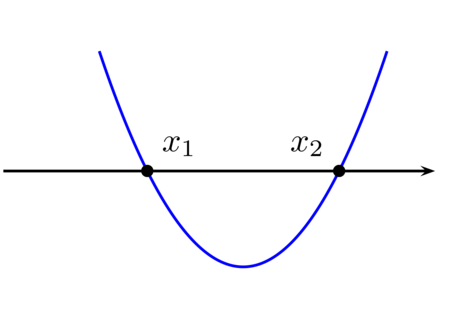
\includegraphics{Picture_FIGLabelFigParaboleHautjOEAznPICTParaboleHautjOEAzn-for_eps.pdf}

            % TODO : regarder comment on peut faire en phystricks que l'image soit produite indépendamment de la figure.
        \end{multicols}
    \item
        Si \( a<0\), alors nous avons le tableau de signe suivant.
        \begin{multicols}{2}
            \begin{equation*}
                \begin{array}[h]{|c||c|c|c|c|c|}
                    \hline
                    x&\ldots&x_1&\ldots&x_2&\ldots\\
                    \hline
                    a&-&-&-&-&-\\
                    \hline
                    x-x_1&-&0&+&+&+\\
                    \hline
                    x-x_2&-&-&-&0&+\\
                    \hline\hline
                    f(x)&-&0&+&0&-\\
                    \hline
                \end{array}
            \end{equation*}
            La parabole étant dirigée vers le bas, il est normal qu'elle soit négative hors de l'intervalle entre les racines, et donc positive entre les racines.

            \columnbreak

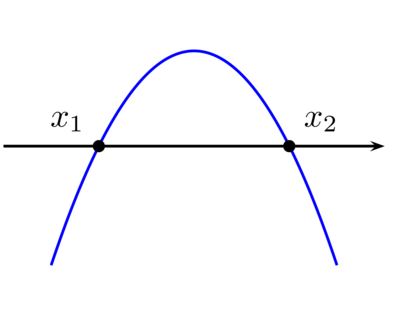
\includegraphics{Picture_FIGLabelFigParaboleBasDqAAuaPICTParaboleBasDqAAua-for_eps.pdf}
        \end{multicols}

\end{enumerate}

\begin{Aretenir}
    Lorsque la parabole \( ax^2+bx+c\) a deux racines distinctes \( x_1<x_2\), elle a le signe de \( a\) hors de l'intervalle entre les racines et le signe opposé à \( a\) entre les deux racines. Le tableau de signe est donc soit
            \begin{equation}
                \begin{array}[h]{|c||c|c|c|c|c|}
                    \hline
                    x&\ldots&x_1&\ldots&x_2&\ldots\\
                    \hline
                    f(x)&+&0&-&0&+\\
                    \hline
                \end{array}
            \end{equation}
            pour \( a>0\), soit
            \begin{equation}
                \begin{array}[h]{|c||c|c|c|c|c|}
                    \hline
                    x&\ldots&x_1&\ldots&x_2&\ldots\\
                    \hline
                    f(x)&-&0&+&0&-\\
                    \hline
                \end{array}
            \end{equation}
            pour \( a<0\).

            Attention : il prendre soin à trier les racines dans l'ordre croissant avant de créer le tableau de signe.
\end{Aretenir}

%///////////////////////////////////////////////////////////////////////////////////////////////////////////////////////////
\subsubsection{Une seule racine}
%///////////////////////////////////////////////////////////////////////////////////////////////////////////////////////////

Lorsque la parabole possède une unique racine (c'est à dire si le discriminant est nul), le tableau de signe est plus simple. Nous notons \( x_0\) la racine. Le polynôme \( f(x)=ax^2+bx+c\) se factorise en
\begin{equation}
    f(x)=a(x-x_0)^2
\end{equation}
et a donc toujours le signe de \( a\), sauf en \( x=x_0\) où la polynôme s'annule.

\begin{Aretenir}
\begin{enumerate}
    \item
        Si \( a>0\) alors le tableau de signe est
        \begin{multicols}{2}

            \begin{equation*}
                \begin{array}[h]{|c||c|c|c|}
                    \hline
                    x&\ldots&x_0&\ldots\\
                    \hline\hline
                    f(x)&+&0&+\\
                    \hline
                \end{array}
            \end{equation*}
            
            \columnbreak

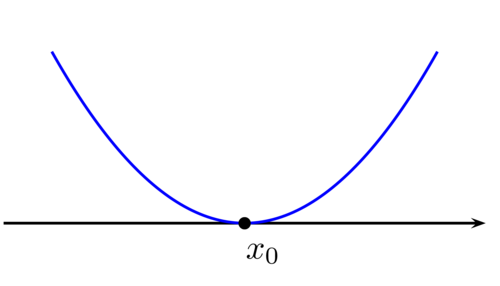
\includegraphics{Picture_FIGLabelFigParaboleUniqueHautviflbYPICTParaboleUniqueHautviflbY-for_eps.pdf}

        \end{multicols}
    \item
        Si \( a<0\) alors le tableau de signe est
        \begin{multicols}{2}

            \begin{equation*}
                \begin{array}[h]{|c||c|c|c|}
                    \hline
                    x&\ldots&x_0&\ldots\\
                    \hline\hline
                    f(x)&-&0&-\\
                    \hline
                \end{array}
            \end{equation*}
            
            \columnbreak
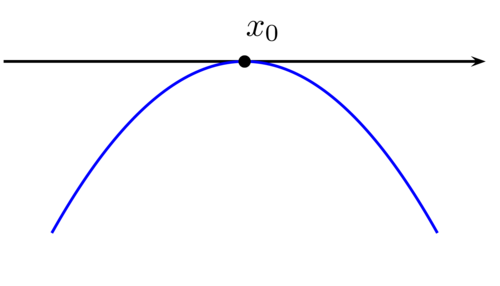
\includegraphics{Picture_FIGLabelFigParaboleUniqueBaskGdqdaPICTParaboleUniqueBaskGdqda-for_eps.pdf}

        \end{multicols}
        
\end{enumerate}
\end{Aretenir}

%///////////////////////////////////////////////////////////////////////////////////////////////////////////////////////////
\subsubsection{Si il n'y a aucune racines}
%///////////////////////////////////////////////////////////////////////////////////////////////////////////////////////////

\begin{Aretenir}
    Si le discriminant \( \Delta=b^2-4ac\) est strictement négatif, alors le polynôme a toujours le signe de \( a\).
\end{Aretenir}

%+++++++++++++++++++++++++++++++++++++++++++++++++++++++++++++++++++++++++++++++++++++++++++++++++++++++++++++++++++++++++++
\section{Résumé de tout ce qu'il faut savoir}
%+++++++++++++++++++++++++++++++++++++++++++++++++++++++++++++++++++++++++++++++++++++++++++++++++++++++++++++++++++++++++++

\begin{multicols}{2}
Une parabole
\begin{equation*}
    f(x)=ax^2+bx+c
\end{equation*}
se présente toujours sous une forme qui ressemble au dessin ci-contre. Les deux racines sont données par les formules
\begin{equation*}
    \begin{aligned}[]
        x_1&=\frac{ -b+\sqrt{\Delta} }{ 2a }&&x_2&=\frac{ -b-\sqrt{\Delta} }{ 2a }
    \end{aligned}
\end{equation*}
où
\begin{equation*}
    \Delta=b^2-4ac.
\end{equation*}

%The result is on figure \ref{LabelFigParaboleResumeHNiyfR}. % From file ParaboleResumeHNiyfR
%\newcommand{\CaptionFigParaboleResumeHNiyfR}{<+Type your caption here+>}
\columnbreak
\input{Fig_ParaboleResumeHNiyfR.pstricks}
\end{multicols}
<++>



%+++++++++++++++++++++++++++++++++++++++++++++++++++++++++++++++++++++++++++++++++++++++++++++++++++++++++++++++++++++++++++
\section{Exercices sur le second degré}
%+++++++++++++++++++++++++++++++++++++++++++++++++++++++++++++++++++++++++++++++++++++++++++++++++++++++++++++++++++++++++++

%---------------------------------------------------------------------------------------------------------------------------
\subsection{Tableau de signe et inéquations connaissant une factorisation}
%---------------------------------------------------------------------------------------------------------------------------

\Exo{Premiere-0030}
\Exo{Premiere-0063}
\Exo{Premiere-0062}
\Exo{Premiere-0024}                                                                                                                                  
\Exo{Premiere-0061}

%---------------------------------------------------------------------------------------------------------------------------
\subsection{Trouver des paraboles vérifiant certaines conditions}
%---------------------------------------------------------------------------------------------------------------------------

\Exo{Premiere-0031}
\Exo{Premiere-0041}

%---------------------------------------------------------------------------------------------------------------------------
\subsection{Lecture de graphiques}
%---------------------------------------------------------------------------------------------------------------------------


\Exo{Premiere-0032}
\Exo{Premiere-0059}
\Exo{Premiere-0060}
\Exo{Premiere-0040}

%---------------------------------------------------------------------------------------------------------------------------
\subsection{Résolution}
%---------------------------------------------------------------------------------------------------------------------------

% Résolution

\Exo{Premiere-0069}
\Exo{Premiere-0046}

%---------------------------------------------------------------------------------------------------------------------------
\subsection{Factorisation}
%---------------------------------------------------------------------------------------------------------------------------

\Exo{Premiere-0047}

%---------------------------------------------------------------------------------------------------------------------------
\subsection{Problèmes}
%---------------------------------------------------------------------------------------------------------------------------

\Exo{Premiere-0044}
\Exo{Premiere-0025}                                                                                                                                   
\Exo{Premiere-0028}
\Exo{Premiere-0029}
\Exo{Premiere-0045}

%---------------------------------------------------------------------------------------------------------------------------
\subsection{Équations sans terme indépendant}
%---------------------------------------------------------------------------------------------------------------------------
% Je ne sais pas si il faut laisser ces exercices ici...

\Exo{Premiere-0042}
\Exo{Premiere-0026}                                                                                               
\Exo{Premiere-0043}
\Exo{Seconde-0052}
